\subsection{Question 1}
\begin{figure}[H]
  \centering
  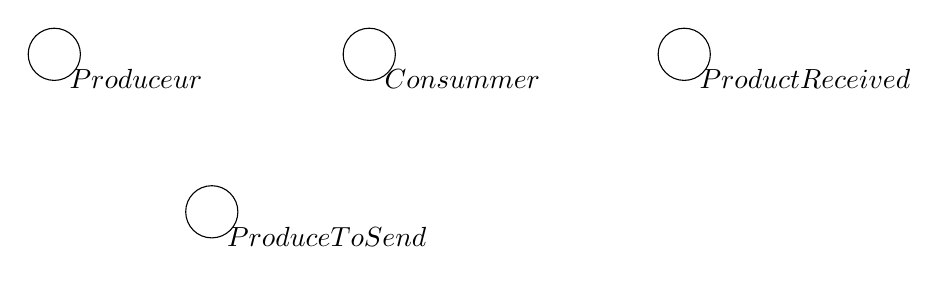
\begin{tikzpicture}

    \draw (-6,2) node[below right = 2pt] {$Produceur$};
    \node[draw,circle,scale=2] (P) at (-6, 2) {};
    \draw (-2,2) node[below right = 2pt] {$Consummer$};
    \node[draw,circle,scale=2] (C) at (-2, 2) {};
    \draw (-4,0) node[below right = 2pt] {$ProduceToSend$};
    \node[draw,circle,scale=2] (PtS) at (-4,0) {};
    \draw (2,2) node[below right = 2pt] {$ProductReceived$};
    \node[draw,circle,scale=2] (PR) at (2, 2) {}; %%

    \end{tikzpicture}
  \caption{Réseau de petri associé à l'exercice 5} \label{fig:M5}
\end{figure}

\subsection{Question 2}

\subsection{Question 3}